% Created by tikzDevice version 0.12 on 2019-03-22 14:21:55
% !TEX encoding = UTF-8 Unicode
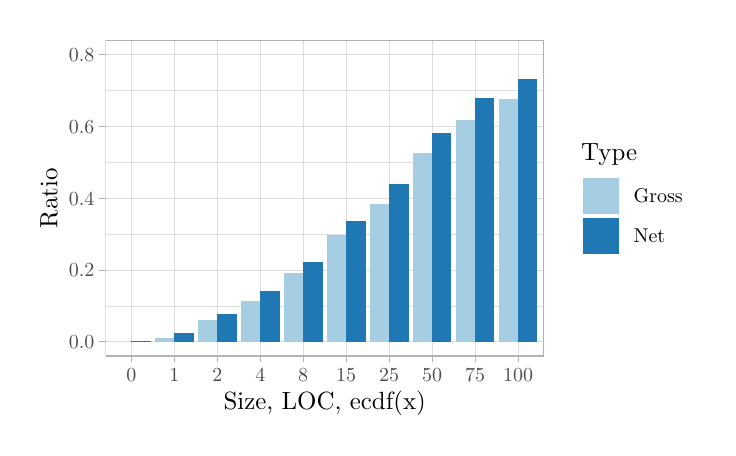
\begin{tikzpicture}[x=1pt,y=1pt]
\definecolor{fillColor}{RGB}{255,255,255}
\path[use as bounding box,fill=fillColor,fill opacity=0.00] (0,0) rectangle (245.72,144.54);
\begin{scope}
\path[clip] (  0.00,  0.00) rectangle (245.72,144.54);
\definecolor{drawColor}{RGB}{255,255,255}
\definecolor{fillColor}{RGB}{255,255,255}

\path[draw=drawColor,line width= 0.5pt,line join=round,line cap=round,fill=fillColor] (  0.00,  0.00) rectangle (245.72,144.54);
\end{scope}
\begin{scope}
\path[clip] ( 28.14, 25.85) rectangle (186.52,140.04);
\definecolor{fillColor}{RGB}{255,255,255}

\path[fill=fillColor] ( 28.14, 25.85) rectangle (186.52,140.04);
\definecolor{drawColor}{gray}{0.87}

\path[draw=drawColor,line width= 0.1pt,line join=round] ( 28.14, 44.01) --
	(186.52, 44.01);

\path[draw=drawColor,line width= 0.1pt,line join=round] ( 28.14, 69.97) --
	(186.52, 69.97);

\path[draw=drawColor,line width= 0.1pt,line join=round] ( 28.14, 95.92) --
	(186.52, 95.92);

\path[draw=drawColor,line width= 0.1pt,line join=round] ( 28.14,121.87) --
	(186.52,121.87);

\path[draw=drawColor,line width= 0.2pt,line join=round] ( 28.14, 31.04) --
	(186.52, 31.04);

\path[draw=drawColor,line width= 0.2pt,line join=round] ( 28.14, 56.99) --
	(186.52, 56.99);

\path[draw=drawColor,line width= 0.2pt,line join=round] ( 28.14, 82.94) --
	(186.52, 82.94);

\path[draw=drawColor,line width= 0.2pt,line join=round] ( 28.14,108.90) --
	(186.52,108.90);

\path[draw=drawColor,line width= 0.2pt,line join=round] ( 28.14,134.85) --
	(186.52,134.85);

\path[draw=drawColor,line width= 0.2pt,line join=round] ( 37.46, 25.85) --
	( 37.46,140.04);

\path[draw=drawColor,line width= 0.2pt,line join=round] ( 52.98, 25.85) --
	( 52.98,140.04);

\path[draw=drawColor,line width= 0.2pt,line join=round] ( 68.51, 25.85) --
	( 68.51,140.04);

\path[draw=drawColor,line width= 0.2pt,line join=round] ( 84.04, 25.85) --
	( 84.04,140.04);

\path[draw=drawColor,line width= 0.2pt,line join=round] ( 99.57, 25.85) --
	( 99.57,140.04);

\path[draw=drawColor,line width= 0.2pt,line join=round] (115.09, 25.85) --
	(115.09,140.04);

\path[draw=drawColor,line width= 0.2pt,line join=round] (130.62, 25.85) --
	(130.62,140.04);

\path[draw=drawColor,line width= 0.2pt,line join=round] (146.15, 25.85) --
	(146.15,140.04);

\path[draw=drawColor,line width= 0.2pt,line join=round] (161.67, 25.85) --
	(161.67,140.04);

\path[draw=drawColor,line width= 0.2pt,line join=round] (177.20, 25.85) --
	(177.20,140.04);
\definecolor{fillColor}{RGB}{31,120,180}

\path[fill=fillColor] ( 37.46, 31.04) rectangle ( 44.44, 31.49);
\definecolor{fillColor}{RGB}{166,206,227}

\path[fill=fillColor] ( 30.47, 31.04) rectangle ( 37.46, 31.04);
\definecolor{fillColor}{RGB}{31,120,180}

\path[fill=fillColor] ( 52.98, 31.04) rectangle ( 59.97, 34.09);
\definecolor{fillColor}{RGB}{166,206,227}

\path[fill=fillColor] ( 46.00, 31.04) rectangle ( 52.98, 32.28);
\definecolor{fillColor}{RGB}{31,120,180}

\path[fill=fillColor] ( 68.51, 31.04) rectangle ( 75.50, 41.20);
\definecolor{fillColor}{RGB}{166,206,227}

\path[fill=fillColor] ( 61.52, 31.04) rectangle ( 68.51, 38.83);
\definecolor{fillColor}{RGB}{31,120,180}

\path[fill=fillColor] ( 84.04, 31.04) rectangle ( 91.03, 49.33);
\definecolor{fillColor}{RGB}{166,206,227}

\path[fill=fillColor] ( 77.05, 31.04) rectangle ( 84.04, 45.72);
\definecolor{fillColor}{RGB}{31,120,180}

\path[fill=fillColor] ( 99.57, 31.04) rectangle (106.55, 59.84);
\definecolor{fillColor}{RGB}{166,206,227}

\path[fill=fillColor] ( 92.58, 31.04) rectangle ( 99.57, 55.88);
\definecolor{fillColor}{RGB}{31,120,180}

\path[fill=fillColor] (115.09, 31.04) rectangle (122.08, 74.63);
\definecolor{fillColor}{RGB}{166,206,227}

\path[fill=fillColor] (108.11, 31.04) rectangle (115.09, 69.55);
\definecolor{fillColor}{RGB}{31,120,180}

\path[fill=fillColor] (130.62, 31.04) rectangle (137.61, 88.18);
\definecolor{fillColor}{RGB}{166,206,227}

\path[fill=fillColor] (123.63, 31.04) rectangle (130.62, 80.95);
\definecolor{fillColor}{RGB}{31,120,180}

\path[fill=fillColor] (146.15, 31.04) rectangle (153.13,106.59);
\definecolor{fillColor}{RGB}{166,206,227}

\path[fill=fillColor] (139.16, 31.04) rectangle (146.15, 99.25);
\definecolor{fillColor}{RGB}{31,120,180}

\path[fill=fillColor] (161.67, 31.04) rectangle (168.66,119.13);
\definecolor{fillColor}{RGB}{166,206,227}

\path[fill=fillColor] (154.69, 31.04) rectangle (161.67,111.34);
\definecolor{fillColor}{RGB}{31,120,180}

\path[fill=fillColor] (177.20, 31.04) rectangle (184.19,125.90);
\definecolor{fillColor}{RGB}{166,206,227}

\path[fill=fillColor] (170.21, 31.04) rectangle (177.20,118.79);
\definecolor{drawColor}{gray}{0.70}

\path[draw=drawColor,line width= 0.5pt,line join=round,line cap=round] ( 28.14, 25.85) rectangle (186.52,140.04);
\end{scope}
\begin{scope}
\path[clip] (  0.00,  0.00) rectangle (245.72,144.54);
\definecolor{drawColor}{gray}{0.30}

\node[text=drawColor,anchor=base east,inner sep=0pt, outer sep=0pt, scale=  0.72] at ( 24.09, 28.56) {0.0};

\node[text=drawColor,anchor=base east,inner sep=0pt, outer sep=0pt, scale=  0.72] at ( 24.09, 54.51) {0.2};

\node[text=drawColor,anchor=base east,inner sep=0pt, outer sep=0pt, scale=  0.72] at ( 24.09, 80.46) {0.4};

\node[text=drawColor,anchor=base east,inner sep=0pt, outer sep=0pt, scale=  0.72] at ( 24.09,106.42) {0.6};

\node[text=drawColor,anchor=base east,inner sep=0pt, outer sep=0pt, scale=  0.72] at ( 24.09,132.37) {0.8};
\end{scope}
\begin{scope}
\path[clip] (  0.00,  0.00) rectangle (245.72,144.54);
\definecolor{drawColor}{gray}{0.70}

\path[draw=drawColor,line width= 0.2pt,line join=round] ( 25.89, 31.04) --
	( 28.14, 31.04);

\path[draw=drawColor,line width= 0.2pt,line join=round] ( 25.89, 56.99) --
	( 28.14, 56.99);

\path[draw=drawColor,line width= 0.2pt,line join=round] ( 25.89, 82.94) --
	( 28.14, 82.94);

\path[draw=drawColor,line width= 0.2pt,line join=round] ( 25.89,108.90) --
	( 28.14,108.90);

\path[draw=drawColor,line width= 0.2pt,line join=round] ( 25.89,134.85) --
	( 28.14,134.85);
\end{scope}
\begin{scope}
\path[clip] (  0.00,  0.00) rectangle (245.72,144.54);
\definecolor{drawColor}{gray}{0.70}

\path[draw=drawColor,line width= 0.2pt,line join=round] ( 37.46, 23.60) --
	( 37.46, 25.85);

\path[draw=drawColor,line width= 0.2pt,line join=round] ( 52.98, 23.60) --
	( 52.98, 25.85);

\path[draw=drawColor,line width= 0.2pt,line join=round] ( 68.51, 23.60) --
	( 68.51, 25.85);

\path[draw=drawColor,line width= 0.2pt,line join=round] ( 84.04, 23.60) --
	( 84.04, 25.85);

\path[draw=drawColor,line width= 0.2pt,line join=round] ( 99.57, 23.60) --
	( 99.57, 25.85);

\path[draw=drawColor,line width= 0.2pt,line join=round] (115.09, 23.60) --
	(115.09, 25.85);

\path[draw=drawColor,line width= 0.2pt,line join=round] (130.62, 23.60) --
	(130.62, 25.85);

\path[draw=drawColor,line width= 0.2pt,line join=round] (146.15, 23.60) --
	(146.15, 25.85);

\path[draw=drawColor,line width= 0.2pt,line join=round] (161.67, 23.60) --
	(161.67, 25.85);

\path[draw=drawColor,line width= 0.2pt,line join=round] (177.20, 23.60) --
	(177.20, 25.85);
\end{scope}
\begin{scope}
\path[clip] (  0.00,  0.00) rectangle (245.72,144.54);
\definecolor{drawColor}{gray}{0.30}

\node[text=drawColor,anchor=base,inner sep=0pt, outer sep=0pt, scale=  0.72] at ( 37.46, 16.84) {0};

\node[text=drawColor,anchor=base,inner sep=0pt, outer sep=0pt, scale=  0.72] at ( 52.98, 16.84) {1};

\node[text=drawColor,anchor=base,inner sep=0pt, outer sep=0pt, scale=  0.72] at ( 68.51, 16.84) {2};

\node[text=drawColor,anchor=base,inner sep=0pt, outer sep=0pt, scale=  0.72] at ( 84.04, 16.84) {4};

\node[text=drawColor,anchor=base,inner sep=0pt, outer sep=0pt, scale=  0.72] at ( 99.57, 16.84) {8};

\node[text=drawColor,anchor=base,inner sep=0pt, outer sep=0pt, scale=  0.72] at (115.09, 16.84) {15};

\node[text=drawColor,anchor=base,inner sep=0pt, outer sep=0pt, scale=  0.72] at (130.62, 16.84) {25};

\node[text=drawColor,anchor=base,inner sep=0pt, outer sep=0pt, scale=  0.72] at (146.15, 16.84) {50};

\node[text=drawColor,anchor=base,inner sep=0pt, outer sep=0pt, scale=  0.72] at (161.67, 16.84) {75};

\node[text=drawColor,anchor=base,inner sep=0pt, outer sep=0pt, scale=  0.72] at (177.20, 16.84) {100};
\end{scope}
\begin{scope}
\path[clip] (  0.00,  0.00) rectangle (245.72,144.54);
\definecolor{drawColor}{RGB}{0,0,0}

\node[text=drawColor,anchor=base,inner sep=0pt, outer sep=0pt, scale=  0.90] at (107.33,  6.44) {Size, LOC, ecdf(x)};
\end{scope}
\begin{scope}
\path[clip] (  0.00,  0.00) rectangle (245.72,144.54);
\definecolor{drawColor}{RGB}{0,0,0}

\node[text=drawColor,rotate= 90.00,anchor=base,inner sep=0pt, outer sep=0pt, scale=  0.90] at ( 10.70, 82.94) {Ratio};
\end{scope}
\begin{scope}
\path[clip] (  0.00,  0.00) rectangle (245.72,144.54);
\definecolor{fillColor}{RGB}{255,255,255}

\path[fill=fillColor] (195.52, 57.67) rectangle (241.22,108.22);
\end{scope}
\begin{scope}
\path[clip] (  0.00,  0.00) rectangle (245.72,144.54);
\definecolor{drawColor}{RGB}{0,0,0}

\node[text=drawColor,anchor=base west,inner sep=0pt, outer sep=0pt, scale=  0.90] at (200.02, 96.55) {Type};
\end{scope}
\begin{scope}
\path[clip] (  0.00,  0.00) rectangle (245.72,144.54);
\definecolor{fillColor}{RGB}{255,255,255}

\path[fill=fillColor] (200.02, 76.62) rectangle (214.47, 91.08);
\end{scope}
\begin{scope}
\path[clip] (  0.00,  0.00) rectangle (245.72,144.54);
\definecolor{fillColor}{RGB}{166,206,227}

\path[fill=fillColor] (200.73, 77.33) rectangle (213.76, 90.36);
\end{scope}
\begin{scope}
\path[clip] (  0.00,  0.00) rectangle (245.72,144.54);
\definecolor{fillColor}{RGB}{255,255,255}

\path[fill=fillColor] (200.02, 62.17) rectangle (214.47, 76.62);
\end{scope}
\begin{scope}
\path[clip] (  0.00,  0.00) rectangle (245.72,144.54);
\definecolor{fillColor}{RGB}{31,120,180}

\path[fill=fillColor] (200.73, 62.88) rectangle (213.76, 75.91);
\end{scope}
\begin{scope}
\path[clip] (  0.00,  0.00) rectangle (245.72,144.54);
\definecolor{drawColor}{RGB}{0,0,0}

\node[text=drawColor,anchor=base west,inner sep=0pt, outer sep=0pt, scale=  0.72] at (218.97, 81.37) {Gross};
\end{scope}
\begin{scope}
\path[clip] (  0.00,  0.00) rectangle (245.72,144.54);
\definecolor{drawColor}{RGB}{0,0,0}

\node[text=drawColor,anchor=base west,inner sep=0pt, outer sep=0pt, scale=  0.72] at (218.97, 66.91) {Net};
\end{scope}
\end{tikzpicture}
